\section{Introducción}

El presente trabajo practico tiene como objetivo aprender a utilizar instrucciones que operan con múltiples datos SIMD (Single instruction, multiple data), soportada por la familia de procesadores x86-64 de Intel. En general, este tipo de instrucciones se utilizan mucho en procesamiento digital de señales y procesamiento de gráficos. Debido a restricciones de la cátedra, solo utilizaremos SSE (Streaming SIMD Extensions) y no el conjunto de instrucciones mas nuevo AVX (Advanced Vector Extensions).
 
\subsection{Historia}
 
\begin{wrapfigure}{r}{0.3\textwidth}
  \begin{center}
    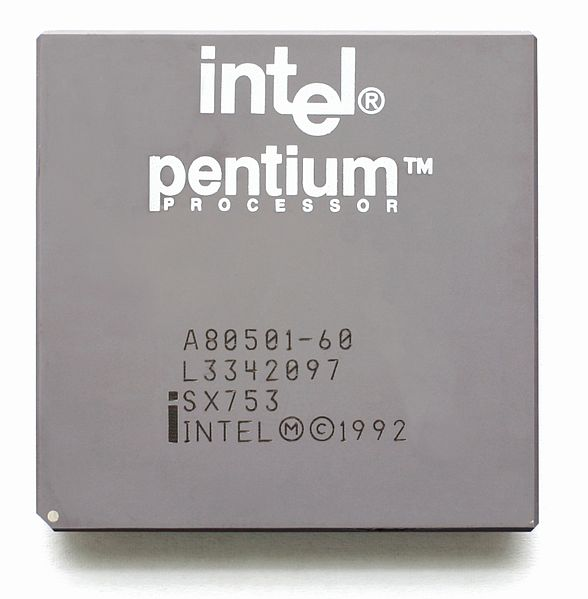
\includegraphics[scale=0.2]{pentium.jpg}
  \end{center}
  \caption{Intel Pentium P5}
  \begin{center}
    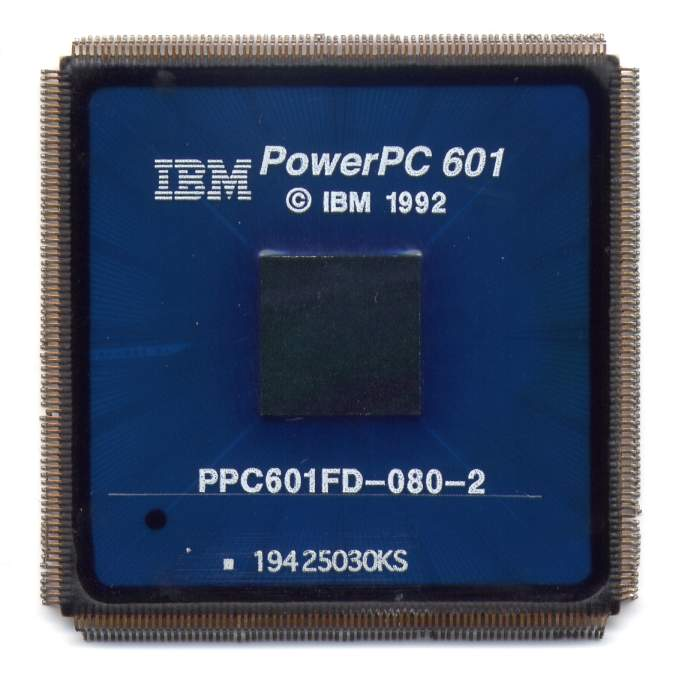
\includegraphics[scale=1.5]{powerpc.jpg}
  \end{center}
  \caption{Power PC}
\end{wrapfigure} 
 
El conjunto de instrucciones MMX (MultiMedia eXtension) fue el primero en implementar SIMD en la arquitectura Intel en el año 1997, con los procesadores Pentium II. La idea era, como lo indica el nombre, permitir el procesamiento de operaciones sobre múltiples datos en simultaneo. Esto en general se conoce como paralelismo a nivel de datos, donde un único proceso es capaz de ejecutar estas instrucciones.

MMX define 8 nuevos registros de 64 bits, desde el MM0 al MM7. A nivel arquitectura, estos registros eran simplemente un alias de los registros de la FPU, por lo que cualquier operación en la FPU afecta a los registros MM$i$.

En el año 1999, con el objetivo de responder a las mejoras introducidas por la competencia, en general por el AltiVec en las PowerPc de Motorola y el sistema POWER de IBM, Intel introduce el conjunto de instrucciones SSE con la serie de procesadores Pentium III. El conjunto de instrucciones SSE tenia 70 nuevas instrucciones. Aquí Intel agrega 8 nuevos registros de 128 bits, XMM0 a XMM7, independientes de la FPU. Este conjunto de instrucciones luego se actualizo con SSE2 (2001), SSE3 (2004), SSSE3 (2006) y SSE4(2006).

En el año 2011 finalmente se introduce al mercado las extensiones al conjunto de instrucciones AVX (Advanced Vector Extensions), primero implementado por la linea de procesadores de Intel Sandy Bridge. AVX expande el tamaño de los registros de 128 a 256 bits, y se renombra a estos registros como YMM0-YMM7. Introduce las operaciones vectorizadas de tres operandos. 

Intel introduce AVX2 en el año 2013 con la linea de procesadores Haswell, que expande muchas de las instrucciones de SSE y AVX a 256 bits.

Actualmente Intel esta por lanzar este año la linea de procesadores Xeon Phi Knights Landing, que busca expandir las operaciones y los registros de AVX2 a 512 bits.

\subsection{Filtros de Imágenes}

Una aplicación típica de este tipo de instrucciones es el procesamiento de imágenes. Esto se debe a que una imagen esta representada por un mapa de píxeles, y en general al procesar imágenes se esta llevando a cabo el mismo tipo de procedimiento muchas veces. A continuación se analizaremos algunos filtros de imágenes, técnicas de implementación de los mismos, y haremos un análisis cuantitativo de las diferencias entre ellos, así como posibles mejoras y reflexiones respecto de las implementaciones puntuales.

A fines de simplificar el análisis, solo utilizaremos imágenes de tamaño $HxW$ en formato bmp, tal que $w$ sea múltiplo de 4. Notaremos a $i$ como el índice de las filas, a $j$ como el índice de las columnas y a $k$ como el índice de los componentes de color de cada píxel. $m_{i, j, k}$ por lo tanto sera el componente $k$ del píxel asociado a la fila $i$, columna $j$.
